\chapter{\glsentryshort{dune} \glsentryshort{nd} Event Pile-up Study Data}
\label{chap:pile-up-data}

\section{\SI{2}{\mega\watt} Beam at \SI{80}{\giga\electronvolt} Proton Energy}

\begin{figure}[htb]
	\centering
	\includegraphics[width=\textwidth]{pile-up/2MW/abs_2d_missed}
	\caption[Pile-up study missed vs.\ true photon energy, \SI{2}{\mega\watt} beam]{%
		Missed energy versus true photon energy for a simple \Pgpz-induced \acrshort{em} shower reconstruction algorithm based on a cone-cylinder union.
		All energy deposited outside of the cone-cylinder union is counted as missed.
		\SI{2}{\mega\watt} beam of \SI{80}{\giga\electronvolt} protons.
		Entries: Central cell shows plotted entries, other cells show overflow entries in direction w.r.t.\ central cell.
	}
\end{figure}

\begin{figure}[htb]
	\centering
	\includegraphics[width=\textwidth]{pile-up/2MW/missed_abs_x}
	\caption[Pile-up study mean missed vs.\ true photon energy, \SI{2}{\mega\watt} beam]{%
		Mean missed energy versus true photon energy for a simple \Pgpz-induced \acrshort{em} shower reconstruction algorithm based on a cone-cylinder union.
		All energy deposited outside of the cone-cylinder union is counted as missed.
		\SI{2}{\mega\watt} beam of \SI{80}{\giga\electronvolt} protons.
	}
\end{figure}

\begin{figure}[htb]
	\centering
	\includegraphics[width=\textwidth]{pile-up/2MW/rel_2d_missed}
	\caption[Pile-up study missed fractional vs.\ true photon energy, \SI{2}{\mega\watt} beam]{%
		Missed energy fraction versus true photon energy for a simple \Pgpz-induced \acrshort{em} shower reconstruction algorithm based on a cone-cylinder union.
		All energy deposited outside of the cone-cylinder union is counted as missed.
		\SI{2}{\mega\watt} beam of \SI{80}{\giga\electronvolt} protons.
		Entries: Central cell shows plotted entries, other cells show overflow entries in direction w.r.t.\ central cell.
	}
\end{figure}

\begin{figure}[htb]
	\centering
	\includegraphics[width=\textwidth]{pile-up/2MW/missed_rel_x}
	\caption[Pile-up study mean missed fractional vs.\ true photon energy, \SI{2}{\mega\watt} beam]{%
		Mean missed energy fraction versus true photon energy for a simple \Pgpz-induced \acrshort{em} shower reconstruction algorithm based on a cone-cylinder union.
		All energy deposited outside of the cone-cylinder union is counted as missed.
		\SI{2}{\mega\watt} beam of \SI{80}{\giga\electronvolt} protons.
	}
\end{figure}

\begin{figure}[htb]
	\centering
	\includegraphics[width=\textwidth]{pile-up/2MW/missed_rel_y}
	\caption[Pile-up study photon vs.\ missed energy fraction, \SI{2}{\mega\watt} beam]{%
		Cumulative fraction of photons versus missed energy fraction for a simple \Pgpz-induced \acrshort{em} shower reconstruction algorithm based on a cone-cylinder union.
		All energy deposited outside of the cone-cylinder union is counted as missed.
		The curve depicts the fraction of photons on the y-axis with a missed energy fraction equal to or lower than the corresponding value on the x-axis.
		\SI{2}{\mega\watt} beam of \SI{80}{\giga\electronvolt} protons.
	}
\end{figure}

\begin{figure}[htb]
	\centering
	\includegraphics[width=\textwidth]{pile-up/2MW/abs_2d_other}
	\caption[Pile-up study misidentified vs.\ true neutrino energy, \SI{2}{\mega\watt} beam]{%
		Misidentified energy versus true neutrino energy for a simple \Pgpz-induced \acrshort{em} shower reconstruction algorithm based on a cone-cylinder union.
		All energy deposited inside the cone-cylinder union by descendants of neutrinos different from the parent of the corresponding \Pgpz photon is counted as misidentified.
		\SI{2}{\mega\watt} beam of \SI{80}{\giga\electronvolt} protons.
		Entries: Central cell shows plotted entries, other cells show overflow entries in direction w.r.t.\ central cell.
	}
\end{figure}

\begin{figure}[htb]
	\centering
	\includegraphics[width=\textwidth]{pile-up/2MW/abs_2d_notmu}
	\caption[Pile-up study misidentified vs.\ true neutrino energy, no muons, \SI{2}{\mega\watt} beam]{%
		Misidentified energy versus true neutrino energy for a simple \Pgpz-induced \acrshort{em} shower reconstruction algorithm based on a cone-cylinder union.
		Energy deposited inside the cone-cylinder union by descendants of neutrinos different from the parent of the corresponding \Pgpz photon is counted as misidentified.
		Any energy deposited by muons is excluded.
		\SI{2}{\mega\watt} beam of \SI{80}{\giga\electronvolt} protons.
		Entries: Central cell shows plotted entries, other cells show overflow entries in direction w.r.t.\ central cell.
	}
\end{figure}

\begin{figure}[htb]
	\centering
	\includegraphics[width=\textwidth]{pile-up/2MW/abs_2d_neutral}
	\caption[Pile-up study misidentified vs.\ true neutrino energy, only neutrals, \SI{2}{\mega\watt} beam]{%
		Misidentified energy versus true neutrino energy for a simple \Pgpz-induced \acrshort{em} shower reconstruction algorithm based on a cone-cylinder union.
		Energy deposited inside the cone-cylinder union by descendants of neutrinos different from the parent of the corresponding \Pgpz photon is counted as misidentified.
		Only energy deposited by photons, neutrons, or any of their descendants is included.
		\SI{2}{\mega\watt} beam of \SI{80}{\giga\electronvolt} protons.
		Entries: Central cell shows plotted entries, other cells show overflow entries in direction w.r.t.\ central cell.
	}
\end{figure}

\begin{figure}[htb]
	\centering
	\includegraphics[width=\textwidth]{pile-up/2MW/misid_abs_x}
	\caption[Pile-up study mean misidentified vs.\ true neutrino energy, \SI{2}{\mega\watt} beam]{%
		Mean misidentified energy versus true neutrino energy for a simple \Pgpz-induced \acrshort{em} shower reconstruction algorithm based on a cone-cylinder union.
		All energy deposited inside the cone-cylinder union by descendants of neutrinos different from the parent of the corresponding \Pgpz photon is counted as misidentified.
		Colour indicates different selections of misidentified energy: total (cyan); excluding depositions from muons (red); deposition from photons, neutrons, and their descendants only (blue).
		\SI{2}{\mega\watt} beam of \SI{80}{\giga\electronvolt} protons.
	}
\end{figure}

\begin{figure}[htb]
	\centering
	\includegraphics[width=\textwidth]{pile-up/2MW/rel_2d_other}
	\caption[Pile-up study misidentified fractional vs.\ true neutrino energy, \SI{2}{\mega\watt} beam]{%
		Misidentified energy fraction versus true neutrino energy for a simple \Pgpz-induced \acrshort{em} shower reconstruction algorithm based on a cone-cylinder union.
		All energy deposited inside the cone-cylinder union by descendants of neutrinos different from the parent of the corresponding \Pgpz photon is counted as misidentified.
		\SI{2}{\mega\watt} beam of \SI{80}{\giga\electronvolt} protons.
		Entries: Central cell shows plotted entries, other cells show overflow entries in direction w.r.t.\ central cell.
	}
\end{figure}

\begin{figure}[htb]
	\centering
	\includegraphics[width=\textwidth]{pile-up/2MW/rel_2d_notmu}
	\caption[Pile-up study misidentified fractional vs.\ true neutrino energy, no muons, \SI{2}{\mega\watt} beam]{%
		Misidentified energy fraction versus true neutrino energy for a simple \Pgpz-induced \acrshort{em} shower reconstruction algorithm based on a cone-cylinder union.
		Energy deposited inside the cone-cylinder union by descendants of neutrinos different from the parent of the corresponding \Pgpz photon is counted as misidentified.
		Any energy deposited by muons is excluded.
		\SI{2}{\mega\watt} beam of \SI{80}{\giga\electronvolt} protons.
		Entries: Central cell shows plotted entries, other cells show overflow entries in direction w.r.t.\ central cell.
	}
\end{figure}

\begin{figure}[htb]
	\centering
	\includegraphics[width=\textwidth]{pile-up/2MW/rel_2d_neutral}
	\caption[Pile-up study misidentified fractional vs.\ true neutrino energy, only neutrals, \SI{2}{\mega\watt} beam]{%
		Misidentified energy fraction versus true neutrino energy for a simple \Pgpz-induced \acrshort{em} shower reconstruction algorithm based on a cone-cylinder union.
		Energy deposited inside the cone-cylinder union by descendants of neutrinos different from the parent of the corresponding \Pgpz photon is counted as misidentified.
		Only energy deposited by photons, neutrons, or any of their descendants is included.
		\SI{2}{\mega\watt} beam of \SI{80}{\giga\electronvolt} protons.
		Entries: Central cell shows plotted entries, other cells show overflow entries in direction w.r.t.\ central cell.
	}
\end{figure}

\begin{figure}[htb]
	\centering
	\includegraphics[width=\textwidth]{pile-up/2MW/misid_rel_x}
	\caption[Pile-up study mean misidentified fractional vs.\ true neutrino energy, \SI{2}{\mega\watt} beam]{%
		Mean misidentified energy fraction versus true neutrino energy for a simple \Pgpz-induced \acrshort{em} shower reconstruction algorithm based on a cone-cylinder union.
		All energy deposited inside the cone-cylinder union by descendants of neutrinos different from the parent of the corresponding \Pgpz photon is counted as misidentified.
		Colour indicates different selections of misidentified energy: total (cyan); excluding depositions from muons (red); deposition from photons, neutrons, and their descendants only (blue).
		\SI{2}{\mega\watt} beam of \SI{80}{\giga\electronvolt} protons.
	}
\end{figure}

\begin{figure}[htb]
	\centering
	\includegraphics[width=\textwidth]{pile-up/2MW/misid_rel_y}
	\caption[Pile-up study neutrino vs.\ misidentified energy fraction, \SI{2}{\mega\watt} beam]{%
		Cumulative fraction of neutrinos versus misidentified energy fraction for a simple \Pgpz-induced \acrshort{em} shower reconstruction algorithm based on a cone-cylinder union.
		All energy deposited inside the cone-cylinder union by descendants of neutrinos different from the parent of the corresponding \Pgpz photon is counted as misidentified.
		Colour indicates different selections of misidentified energy: total (cyan); excluding depositions from muons (red); deposition from photons, neutrons, and their descendants only (blue).
		The curve depicts the fraction of neutrinos on the y-axis with a misidentified energy fraction equal to or lower than the corresponding value on the x-axis.
		\SI{2}{\mega\watt} beam of \SI{80}{\giga\electronvolt} protons.
	}
\end{figure}


\section{\SI{2}{\mega\watt} Beam at \SI{80}{\giga\electronvolt} Proton Energy, XZ Projection}

\begin{figure}[htb]
	\centering
	\includegraphics[width=\textwidth]{pile-up/2MW_XZ/abs_2d_missed}
	\caption[Pile-up study missed vs.\ true photon energy, \SI{2}{\mega\watt} beam, XZ projection]{%
		Missed energy versus true photon energy for a simple \Pgpz-induced \acrshort{em} shower reconstruction algorithm based on a cone-cylinder union.
		All energy deposited outside of the cone-cylinder union is counted as missed.
		\SI{2}{\mega\watt} beam of \SI{80}{\giga\electronvolt} protons.
		As a primitive simulation of a \acrshort{2d} wire readout, only X- and Z-coordinates are used for the energy reconstruction.
		Entries: Central cell shows plotted entries, other cells show overflow entries in direction w.r.t.\ central cell.
	}
\end{figure}

\begin{figure}[htb]
	\centering
	\includegraphics[width=\textwidth]{pile-up/2MW_XZ/missed_abs_x}
	\caption[Pile-up study mean missed vs.\ true photon energy, \SI{2}{\mega\watt} beam, XZ projection]{%
		Mean missed energy versus true photon energy for a simple \Pgpz-induced \acrshort{em} shower reconstruction algorithm based on a cone-cylinder union.
		All energy deposited outside of the cone-cylinder union is counted as missed.
		\SI{2}{\mega\watt} beam of \SI{80}{\giga\electronvolt} protons.
		As a primitive simulation of a \acrshort{2d} wire readout, only X- and Z-coordinates are used for the energy reconstruction.
	}
\end{figure}

\begin{figure}[htb]
	\centering
	\includegraphics[width=\textwidth]{pile-up/2MW_XZ/rel_2d_missed}
	\caption[Pile-up study missed fractional vs.\ true photon energy, \SI{2}{\mega\watt} beam, XZ projection]{%
		Missed energy fraction versus true photon energy for a simple \Pgpz-induced \acrshort{em} shower reconstruction algorithm based on a cone-cylinder union.
		All energy deposited outside of the cone-cylinder union is counted as missed.
		\SI{2}{\mega\watt} beam of \SI{80}{\giga\electronvolt} protons.
		As a primitive simulation of a \acrshort{2d} wire readout, only X- and Z-coordinates are used for the energy reconstruction.
		Entries: Central cell shows plotted entries, other cells show overflow entries in direction w.r.t.\ central cell.
	}
\end{figure}

\begin{figure}[htb]
	\centering
	\includegraphics[width=\textwidth]{pile-up/2MW_XZ/missed_rel_x}
	\caption[Pile-up study mean missed fractional vs.\ true photon energy, \SI{2}{\mega\watt} beam, XZ projection]{%
		Mean missed energy fraction versus true photon energy for a simple \Pgpz-induced \acrshort{em} shower reconstruction algorithm based on a cone-cylinder union.
		All energy deposited outside of the cone-cylinder union is counted as missed.
		\SI{2}{\mega\watt} beam of \SI{80}{\giga\electronvolt} protons.
		As a primitive simulation of a \acrshort{2d} wire readout, only X- and Z-coordinates are used for the energy reconstruction.
	}
\end{figure}

\begin{figure}[htb]
	\centering
	\includegraphics[width=\textwidth]{pile-up/2MW_XZ/missed_rel_y}
	\caption[Pile-up study photon vs.\ missed energy fraction, \SI{2}{\mega\watt} beam, XZ projection]{%
		Cumulative fraction of photons versus missed energy fraction for a simple \Pgpz-induced \acrshort{em} shower reconstruction algorithm based on a cone-cylinder union.
		All energy deposited outside of the cone-cylinder union is counted as missed.
		The curve depicts the fraction of photons on the y-axis with a missed energy fraction equal to or lower than the corresponding value on the x-axis.
		\SI{2}{\mega\watt} beam of \SI{80}{\giga\electronvolt} protons.
		As a primitive simulation of a \acrshort{2d} wire readout, only X- and Z-coordinates are used for the energy reconstruction.
	}
\end{figure}

\begin{figure}[htb]
	\centering
	\includegraphics[width=\textwidth]{pile-up/2MW_XZ/abs_2d_other}
	\caption[Pile-up study misidentified vs.\ true neutrino energy, \SI{2}{\mega\watt} beam, XZ projection]{%
		Misidentified energy versus true neutrino energy for a simple \Pgpz-induced \acrshort{em} shower reconstruction algorithm based on a cone-cylinder union.
		All energy deposited inside the cone-cylinder union by descendants of neutrinos different from the parent of the corresponding \Pgpz photon is counted as misidentified.
		\SI{2}{\mega\watt} beam of \SI{80}{\giga\electronvolt} protons.
		As a primitive simulation of a \acrshort{2d} wire readout, only X- and Z-coordinates are used for the energy reconstruction.
		Entries: Central cell shows plotted entries, other cells show overflow entries in direction w.r.t.\ central cell.
	}
\end{figure}

\begin{figure}[htb]
	\centering
	\includegraphics[width=\textwidth]{pile-up/2MW_XZ/abs_2d_notmu}
	\caption[Pile-up study misidentified vs.\ true neutrino energy, no muons, \SI{2}{\mega\watt} beam, XZ projection]{%
		Misidentified energy versus true neutrino energy for a simple \Pgpz-induced \acrshort{em} shower reconstruction algorithm based on a cone-cylinder union.
		Energy deposited inside the cone-cylinder union by descendants of neutrinos different from the parent of the corresponding \Pgpz photon is counted as misidentified.
		Any energy deposited by muons is excluded.
		\SI{2}{\mega\watt} beam of \SI{80}{\giga\electronvolt} protons.
		As a primitive simulation of a \acrshort{2d} wire readout, only X- and Z-coordinates are used for the energy reconstruction.
		Entries: Central cell shows plotted entries, other cells show overflow entries in direction w.r.t.\ central cell.
	}
\end{figure}

\begin{figure}[htb]
	\centering
	\includegraphics[width=\textwidth]{pile-up/2MW_XZ/abs_2d_neutral}
	\caption[Pile-up study misidentified vs.\ true neutrino energy, only neutrals, \SI{2}{\mega\watt} beam, XZ projection]{%
		Misidentified energy versus true neutrino energy for a simple \Pgpz-induced \acrshort{em} shower reconstruction algorithm based on a cone-cylinder union.
		Energy deposited inside the cone-cylinder union by descendants of neutrinos different from the parent of the corresponding \Pgpz photon is counted as misidentified.
		Only energy deposited by photons, neutrons, or any of their descendants is included.
		\SI{2}{\mega\watt} beam of \SI{80}{\giga\electronvolt} protons.
		As a primitive simulation of a \acrshort{2d} wire readout, only X- and Z-coordinates are used for the energy reconstruction.
		Entries: Central cell shows plotted entries, other cells show overflow entries in direction w.r.t.\ central cell.
	}
\end{figure}

\begin{figure}[htb]
	\centering
	\includegraphics[width=\textwidth]{pile-up/2MW_XZ/misid_abs_x}
	\caption[Pile-up study mean misidentified vs.\ true neutrino energy, \SI{2}{\mega\watt} beam, XZ projection]{%
		Mean misidentified energy versus true neutrino energy for a simple \Pgpz-induced \acrshort{em} shower reconstruction algorithm based on a cone-cylinder union.
		All energy deposited inside the cone-cylinder union by descendants of neutrinos different from the parent of the corresponding \Pgpz photon is counted as misidentified.
		Colour indicates different selections of misidentified energy: total (cyan); excluding depositions from muons (red); deposition from photons, neutrons, and their descendants only (blue).
		\SI{2}{\mega\watt} beam of \SI{80}{\giga\electronvolt} protons.
		As a primitive simulation of a \acrshort{2d} wire readout, only X- and Z-coordinates are used for the energy reconstruction.
	}
\end{figure}

\begin{figure}[htb]
	\centering
	\includegraphics[width=\textwidth]{pile-up/2MW_XZ/rel_2d_other}
	\caption[Pile-up study misidentified fractional vs.\ true neutrino energy, \SI{2}{\mega\watt} beam, XZ projection]{%
		Misidentified energy fraction versus true neutrino energy for a simple \Pgpz-induced \acrshort{em} shower reconstruction algorithm based on a cone-cylinder union.
		All energy deposited inside the cone-cylinder union by descendants of neutrinos different from the parent of the corresponding \Pgpz photon is counted as misidentified.
		\SI{2}{\mega\watt} beam of \SI{80}{\giga\electronvolt} protons.
		As a primitive simulation of a \acrshort{2d} wire readout, only X- and Z-coordinates are used for the energy reconstruction.
		Entries: Central cell shows plotted entries, other cells show overflow entries in direction w.r.t.\ central cell.
	}
\end{figure}

\begin{figure}[htb]
	\centering
	\includegraphics[width=\textwidth]{pile-up/2MW_XZ/rel_2d_notmu}
	\caption[Pile-up study misidentified fractional vs.\ true neutrino energy, no muons, \SI{2}{\mega\watt} beam, XZ projection]{%
		Misidentified energy fraction versus true neutrino energy for a simple \Pgpz-induced \acrshort{em} shower reconstruction algorithm based on a cone-cylinder union.
		Energy deposited inside the cone-cylinder union by descendants of neutrinos different from the parent of the corresponding \Pgpz photon is counted as misidentified.
		Any energy deposited by muons is excluded.
		\SI{2}{\mega\watt} beam of \SI{80}{\giga\electronvolt} protons.
		As a primitive simulation of a \acrshort{2d} wire readout, only X- and Z-coordinates are used for the energy reconstruction.
		Entries: Central cell shows plotted entries, other cells show overflow entries in direction w.r.t.\ central cell.
	}
\end{figure}

\begin{figure}[htb]
	\centering
	\includegraphics[width=\textwidth]{pile-up/2MW_XZ/rel_2d_neutral}
	\caption[Pile-up study misidentified fractional vs.\ true neutrino energy, only neutrals, \SI{2}{\mega\watt} beam, XZ projection]{%
		Misidentified energy fraction versus true neutrino energy for a simple \Pgpz-induced \acrshort{em} shower reconstruction algorithm based on a cone-cylinder union.
		Energy deposited inside the cone-cylinder union by descendants of neutrinos different from the parent of the corresponding \Pgpz photon is counted as misidentified.
		Only energy deposited by photons, neutrons, or any of their descendants is included.
		\SI{2}{\mega\watt} beam of \SI{80}{\giga\electronvolt} protons.
		As a primitive simulation of a \acrshort{2d} wire readout, only X- and Z-coordinates are used for the energy reconstruction.
		Entries: Central cell shows plotted entries, other cells show overflow entries in direction w.r.t.\ central cell.
	}
\end{figure}

\begin{figure}[htb]
	\centering
	\includegraphics[width=\textwidth]{pile-up/2MW_XZ/misid_rel_x}
	\caption[Pile-up study mean misidentified fractional vs.\ true neutrino energy, \SI{2}{\mega\watt} beam, XZ projection]{%
		Mean misidentified energy fraction versus true neutrino energy for a simple \Pgpz-induced \acrshort{em} shower reconstruction algorithm based on a cone-cylinder union.
		All energy deposited inside the cone-cylinder union by descendants of neutrinos different from the parent of the corresponding \Pgpz photon is counted as misidentified.
		Colour indicates different selections of misidentified energy: total (cyan); excluding depositions from muons (red); deposition from photons, neutrons, and their descendants only (blue).
		\SI{2}{\mega\watt} beam of \SI{80}{\giga\electronvolt} protons.
		As a primitive simulation of a \acrshort{2d} wire readout, only X- and Z-coordinates are used for the energy reconstruction.
	}
\end{figure}

\begin{figure}[htb]
	\centering
	\includegraphics[width=\textwidth]{pile-up/2MW_XZ/misid_rel_y}
	\caption[Pile-up study neutrino vs.\ misidentified energy fraction, \SI{2}{\mega\watt} beam, XZ projection]{%
		Cumulative fraction of neutrinos versus misidentified energy fraction for a simple \Pgpz-induced \acrshort{em} shower reconstruction algorithm based on a cone-cylinder union.
		All energy deposited inside the cone-cylinder union by descendants of neutrinos different from the parent of the corresponding \Pgpz photon is counted as misidentified.
		Colour indicates different selections of misidentified energy: total (cyan); excluding depositions from muons (red); deposition from photons, neutrons, and their descendants only (blue).
		The curve depicts the fraction of neutrinos on the y-axis with a misidentified energy fraction equal to or lower than the corresponding value on the x-axis.
		\SI{2}{\mega\watt} beam of \SI{80}{\giga\electronvolt} protons.
		As a primitive simulation of a \acrshort{2d} wire readout, only X- and Z-coordinates are used for the energy reconstruction.
	}
\end{figure}


\section{\SI{10}{\mega\watt} Beam at \SI{80}{\giga\electronvolt} Proton Energy}

\begin{figure}[htb]
	\centering
	\includegraphics[width=\textwidth]{pile-up/10MW/abs_2d_missed}
	\caption[Pile-up study missed vs.\ true photon energy, \SI{10}{\mega\watt} beam]{%
		Missed energy versus true photon energy for a simple \Pgpz-induced \acrshort{em} shower reconstruction algorithm based on a cone-cylinder union.
		All energy deposited outside of the cone-cylinder union is counted as missed.
		\SI{10}{\mega\watt} beam of \SI{80}{\giga\electronvolt} protons.
		Entries: Central cell shows plotted entries, other cells show overflow entries in direction w.r.t.\ central cell.
	}
\end{figure}

\begin{figure}[htb]
	\centering
	\includegraphics[width=\textwidth]{pile-up/10MW/missed_abs_x}
	\caption[Pile-up study mean missed vs.\ true photon energy, \SI{10}{\mega\watt} beam]{%
		Mean missed energy versus true photon energy for a simple \Pgpz-induced \acrshort{em} shower reconstruction algorithm based on a cone-cylinder union.
		All energy deposited outside of the cone-cylinder union is counted as missed.
		\SI{10}{\mega\watt} beam of \SI{80}{\giga\electronvolt} protons.
	}
\end{figure}

\begin{figure}[htb]
	\centering
	\includegraphics[width=\textwidth]{pile-up/10MW/rel_2d_missed}
	\caption[Pile-up study missed fractional vs.\ true photon energy, \SI{10}{\mega\watt} beam]{%
		Missed energy fraction versus true photon energy for a simple \Pgpz-induced \acrshort{em} shower reconstruction algorithm based on a cone-cylinder union.
		All energy deposited outside of the cone-cylinder union is counted as missed.
		\SI{10}{\mega\watt} beam of \SI{80}{\giga\electronvolt} protons.
		Entries: Central cell shows plotted entries, other cells show overflow entries in direction w.r.t.\ central cell.
	}
\end{figure}

\begin{figure}[htb]
	\centering
	\includegraphics[width=\textwidth]{pile-up/10MW/missed_rel_x}
	\caption[Pile-up study mean missed fractional vs.\ true photon energy, \SI{10}{\mega\watt} beam]{%
		Mean missed energy fraction versus true photon energy for a simple \Pgpz-induced \acrshort{em} shower reconstruction algorithm based on a cone-cylinder union.
		All energy deposited outside of the cone-cylinder union is counted as missed.
		\SI{10}{\mega\watt} beam of \SI{80}{\giga\electronvolt} protons.
	}
\end{figure}

\begin{figure}[htb]
	\centering
	\includegraphics[width=\textwidth]{pile-up/10MW/missed_rel_y}
	\caption[Pile-up study photon vs.\ missed energy fraction, \SI{10}{\mega\watt} beam]{%
		Cumulative fraction of photons versus missed energy fraction for a simple \Pgpz-induced \acrshort{em} shower reconstruction algorithm based on a cone-cylinder union.
		All energy deposited outside of the cone-cylinder union is counted as missed.
		The curve depicts the fraction of photons on the y-axis with a missed energy fraction equal to or lower than the corresponding value on the x-axis.
		\SI{10}{\mega\watt} beam of \SI{80}{\giga\electronvolt} protons.
	}
\end{figure}

\begin{figure}[htb]
	\centering
	\includegraphics[width=\textwidth]{pile-up/10MW/abs_2d_other}
	\caption[Pile-up study misidentified vs.\ true neutrino energy, \SI{10}{\mega\watt} beam]{%
		Misidentified energy versus true neutrino energy for a simple \Pgpz-induced \acrshort{em} shower reconstruction algorithm based on a cone-cylinder union.
		All energy deposited inside the cone-cylinder union by descendants of neutrinos different from the parent of the corresponding \Pgpz photon is counted as misidentified.
		\SI{10}{\mega\watt} beam of \SI{80}{\giga\electronvolt} protons.
		Entries: Central cell shows plotted entries, other cells show overflow entries in direction w.r.t.\ central cell.
	}
\end{figure}

\begin{figure}[htb]
	\centering
	\includegraphics[width=\textwidth]{pile-up/10MW/abs_2d_notmu}
	\caption[Pile-up study misidentified vs.\ true neutrino energy, no muons, \SI{10}{\mega\watt} beam]{%
		Misidentified energy versus true neutrino energy for a simple \Pgpz-induced \acrshort{em} shower reconstruction algorithm based on a cone-cylinder union.
		Energy deposited inside the cone-cylinder union by descendants of neutrinos different from the parent of the corresponding \Pgpz photon is counted as misidentified.
		Any energy deposited by muons is excluded.
		\SI{10}{\mega\watt} beam of \SI{80}{\giga\electronvolt} protons.
		Entries: Central cell shows plotted entries, other cells show overflow entries in direction w.r.t.\ central cell.
	}
\end{figure}

\begin{figure}[htb]
	\centering
	\includegraphics[width=\textwidth]{pile-up/10MW/abs_2d_neutral}
	\caption[Pile-up study misidentified vs.\ true neutrino energy, only neutrals, \SI{10}{\mega\watt} beam]{%
		Misidentified energy versus true neutrino energy for a simple \Pgpz-induced \acrshort{em} shower reconstruction algorithm based on a cone-cylinder union.
		Energy deposited inside the cone-cylinder union by descendants of neutrinos different from the parent of the corresponding \Pgpz photon is counted as misidentified.
		Only energy deposited by photons, neutrons, or any of their descendants is included.
		\SI{10}{\mega\watt} beam of \SI{80}{\giga\electronvolt} protons.
		Entries: Central cell shows plotted entries, other cells show overflow entries in direction w.r.t.\ central cell.
	}
\end{figure}

\begin{figure}[htb]
	\centering
	\includegraphics[width=\textwidth]{pile-up/10MW/misid_abs_x}
	\caption[Pile-up study mean misidentified vs.\ true neutrino energy, \SI{10}{\mega\watt} beam]{%
		Mean misidentified energy versus true neutrino energy for a simple \Pgpz-induced \acrshort{em} shower reconstruction algorithm based on a cone-cylinder union.
		All energy deposited inside the cone-cylinder union by descendants of neutrinos different from the parent of the corresponding \Pgpz photon is counted as misidentified.
		Colour indicates different selections of misidentified energy: total (cyan); excluding depositions from muons (red); deposition from photons, neutrons, and their descendants only (blue).
		\SI{10}{\mega\watt} beam of \SI{80}{\giga\electronvolt} protons.
	}
\end{figure}

\begin{figure}[htb]
	\centering
	\includegraphics[width=\textwidth]{pile-up/10MW/rel_2d_other}
	\caption[Pile-up study misidentified fractional vs.\ true neutrino energy, \SI{10}{\mega\watt} beam]{%
		Misidentified energy fraction versus true neutrino energy for a simple \Pgpz-induced \acrshort{em} shower reconstruction algorithm based on a cone-cylinder union.
		All energy deposited inside the cone-cylinder union by descendants of neutrinos different from the parent of the corresponding \Pgpz photon is counted as misidentified.
		\SI{10}{\mega\watt} beam of \SI{80}{\giga\electronvolt} protons.
		Entries: Central cell shows plotted entries, other cells show overflow entries in direction w.r.t.\ central cell.
	}
\end{figure}

\begin{figure}[htb]
	\centering
	\includegraphics[width=\textwidth]{pile-up/10MW/rel_2d_notmu}
	\caption[Pile-up study misidentified fractional vs.\ true neutrino energy, no muons, \SI{10}{\mega\watt} beam]{%
		Misidentified energy fraction versus true neutrino energy for a simple \Pgpz-induced \acrshort{em} shower reconstruction algorithm based on a cone-cylinder union.
		Energy deposited inside the cone-cylinder union by descendants of neutrinos different from the parent of the corresponding \Pgpz photon is counted as misidentified.
		Any energy deposited by muons is excluded.
		\SI{10}{\mega\watt} beam of \SI{80}{\giga\electronvolt} protons.
		Entries: Central cell shows plotted entries, other cells show overflow entries in direction w.r.t.\ central cell.
	}
\end{figure}

\begin{figure}[htb]
	\centering
	\includegraphics[width=\textwidth]{pile-up/10MW/rel_2d_neutral}
	\caption[Pile-up study misidentified fractional vs.\ true neutrino energy, only neutrals, \SI{10}{\mega\watt} beam]{%
		Misidentified energy fraction versus true neutrino energy for a simple \Pgpz-induced \acrshort{em} shower reconstruction algorithm based on a cone-cylinder union.
		Energy deposited inside the cone-cylinder union by descendants of neutrinos different from the parent of the corresponding \Pgpz photon is counted as misidentified.
		Only energy deposited by photons, neutrons, or any of their descendants is included.
		\SI{10}{\mega\watt} beam of \SI{80}{\giga\electronvolt} protons.
		Entries: Central cell shows plotted entries, other cells show overflow entries in direction w.r.t.\ central cell.
	}
\end{figure}

\begin{figure}[htb]
	\centering
	\includegraphics[width=\textwidth]{pile-up/10MW/misid_rel_x}
	\caption[Pile-up study mean misidentified fractional vs.\ true neutrino energy, \SI{10}{\mega\watt} beam]{%
		Mean misidentified energy fraction versus true neutrino energy for a simple \Pgpz-induced \acrshort{em} shower reconstruction algorithm based on a cone-cylinder union.
		All energy deposited inside the cone-cylinder union by descendants of neutrinos different from the parent of the corresponding \Pgpz photon is counted as misidentified.
		Colour indicates different selections of misidentified energy: total (cyan); excluding depositions from muons (red); deposition from photons, neutrons, and their descendants only (blue).
		\SI{10}{\mega\watt} beam of \SI{80}{\giga\electronvolt} protons.
	}
\end{figure}

\begin{figure}[htb]
	\centering
	\includegraphics[width=\textwidth]{pile-up/10MW/misid_rel_y}
	\caption[Pile-up study neutrino vs.\ misidentified energy fraction, \SI{10}{\mega\watt} beam]{%
		Cumulative fraction of neutrinos versus misidentified energy fraction for a simple \Pgpz-induced \acrshort{em} shower reconstruction algorithm based on a cone-cylinder union.
		All energy deposited inside the cone-cylinder union by descendants of neutrinos different from the parent of the corresponding \Pgpz photon is counted as misidentified.
		Colour indicates different selections of misidentified energy: total (cyan); excluding depositions from muons (red); deposition from photons, neutrons, and their descendants only (blue).
		The curve depicts the fraction of neutrinos on the y-axis with a misidentified energy fraction equal to or lower than the corresponding value on the x-axis.
		\SI{10}{\mega\watt} beam of \SI{80}{\giga\electronvolt} protons.
	}
\end{figure}